\chapter{Evaluation}

As mentioned in Chapter 4 there is no reliable baseline and one needs to be established first with some basic CNN architectures. Additionally an annotators inter-agreement rate is computed to have a good guess what is realistically possible and how difficult the test set is. Then different architectures will be compared against each other with and without pre-training in order to find out if transfer learning is a valid option for this problem task. \\

The learning rate decay is defined as reducing the learning rate by a factor of 10 every N epochs and holds true for all the experiments: \\

\[ lr = lr * (0.1^{\frac{epoch}{decay}}) \] \\

For the baseline, I used a grid search approach in optimizing the learning rate and the learning rate decay. For all later architectures, I used SigOpt which utilizes bayesian optimization. With SIgOpt I followed the official guideline to run the model for 10 times for every hyperparameter which needs to be optimized. For Alexnet and all state-of-the-art architectures I optimize the following three hyperparameters: \\

\begin{itemize}
  \item learning rate [0.0001 - 0.1]
  \item momentum [0 - 1]
  \item weight\_decay [0.00001 - 0.01]
\end{itemize} 

\quad

Preliminary runs have shown that 50 epochs are long enough to converge as will be shown for every architecture separately. Running for longer did potentially further increase the accuracy of the training set but not of the test set. Sometimes it even degraded slightly due to overfitting to the training data. SigOpt optimization were all conducted with 50 epochs, so were the follow up runs.

The remaining of this chapter is in the following format. I introduce the optimized hyperparameters for each architecture and show the achieved accuracies. I compare the results with transfer learning and discuss the graphs and confusion matrices. For transfer learning a separate optimization with Sigopt is performed, since the hyperparameters need to be different if the starting point of the model is not randomly defined. Then I will attempt to shed some light into what exactly was learned by showing some of the visualizations.








\section{Annotator Inter-Agreement Rate}

The inter-agreement agreement rate gives a score of how much consensus there is between the different raters. Although it cannot be used as a baseline directly since the computation differs from the computation on how the accuracy is computed, it can show how difficult it is to classify the given test samples. For this task 4 raters were recruited a PhD candidate in Computer Science, a PhD candidate in Virology and Immunology, a PhD candidate in History and a Computer Scientist. They were given 168 images to classify into containing asbestos or not. In order to know what to look for, they were given the same (but slightly reduced in number) pre-classified images that were provided by the laboratory with a note explaining the task. They were allowed to switch forward and back between ground truth examples and the unlabeled samples. They were allowed to ask, make a break and take as much time as they saw fit in order to be certain, that they made the best possible decision.\\


\begin{table}[h] \centering
\ra{1.3}
\caption{Inter-agreement rate (Randolph's kappa) of 4 annotators.}
\resizebox{0.8\textwidth}{!}{%
\begin{tabular}{@{}rccc@{}}
\toprule & Overall Agreement & Free-margin kappa & 95\% confidence interval \\
\midrule
Randolph's kappa     & 78.27\%   & 0.57 &  [0.48, 0.65]     \\
\bottomrule
\end{tabular}}
\label{tbl:interagreement}
\end{table}

\quad

Although the overall agreement percentage is at 78.27\% the Randolph's kappa is only at 0.57. The kappa value ranges from -1 (total disagreement below chance) to 1 (total agreement above chance). Kappa values below 0.4 are considered as "poor", values from 0.4 to 0.75  are considered "intermediate to good" and values  above 0.75 are considered "excellent". Therefore the obtained value of 0.57 is between "intermediate" and "good" gives a quality measure of the reached 78.27\%. \\











\section{CNN\_Basic - Baseline}

For the baseline, a simple 3-layered CNN was chosen with three convolutions and no maxpooling. For the activation function, a leaky ReLU is applied after each convolution. A simple grid search is applied to the model as seen in Table \ref{tbl:cnn-basic-baseline}. The best result is achieved with a rather small learning rate of 0.0005 and an lr-decay of 20.\\

\begin{table*}[h]
    \ra{1.3}
    \caption{Accuracy (\%) for several learning rates and lr-decays for CNN\_Basic as a baseline.}
    \centering
    \begin{small}
    \textsc{
      \resizebox{0.99\textwidth}{!}{%
      \begin{tabular}{rcclcclcc}
      \toprule 
      & \multicolumn{2}{c}{Learning-Rate decay: 10} && %
        \multicolumn{2}{c}{Learning-Rate decay: 15} && %
        \multicolumn{2}{c}{Learning-Rate decay: 20} \\
      \cmidrule{2-3} \cmidrule{5-6}  \cmidrule{8-9}
      & learning rate & accuracy  && %
        learning rate & accuracy  && %
        learning rate & accuracy  \\ 
      \midrule
      CNN\_BASIC        & 0.1 & 69.10\%  &&  0.1 & 65.78\% &&  0.1 & 64.78\% \\
      CNN\_BASIC        & 0.05 & 63.46\%  &&  0.05 & 67.44\% && 0.05 & 65.78\% \\
      CNN\_BASIC        & 0.01 & 69.77\%  &&  0.01 & 70.10\% &&  0.01 & 69.77\% \\
      CNN\_BASIC        & 0.005 & 68.44\%  &&  0.005 & 71.43\% &&  0.005 & 72.09\% \\
      CNN\_BASIC        & 0.001 & 72.43\%  &&  0.001 & 70.10\% &&  0.001 & 74.42\% \\
      CNN\_BASIC        & 0.0005 & 73.75\%  &&  0.0005 & 73.42\% &&  \textbf{0.0005} & \textbf{76.74\%} \\
      CNN\_BASIC        & 0.0001 & 68.11\%  &&  0.0001 & 70.76\% &&  0.0001 & 70.43\% \\
    \bottomrule
    \end{tabular}}
    }
    \end{small}
    %\end{center}
    \vspace{-3.9mm}
    \label{tbl:cnn-basic-baseline}
\end{table*}

\quad


These results are much better than expected and should not be that high since the image size is resized to 32x32 pixels. As seen in Figure \ref{fig:cnn-basic} the training accuracy achieves 94.54\% while the validation accuracy achieves 71.42\%. Such a big difference between training accuracy and the final test accuracy of 76.74\% means that the model overfitted strongly to the training data, learning it too well and thus decreasing generalizability. Having the accuracies for validation and test sets near each other is good and means that the validation set is representable of the test set.

\begin{figure}[h]
\centering
\subfigure{
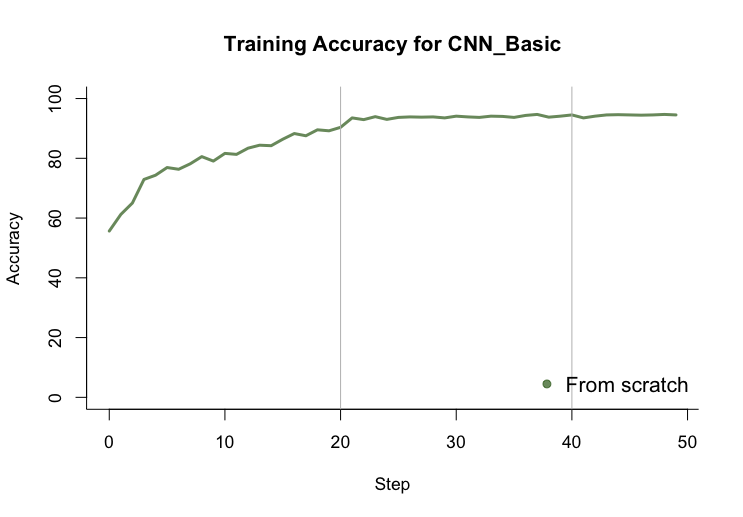
\includegraphics[width=.48\textwidth]{images/chapter5/TrainAccuracy.png}
}
\subfigure{
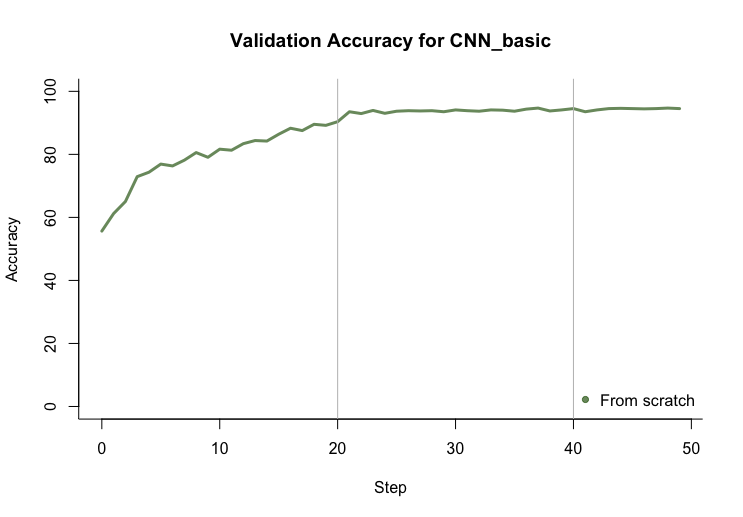
\includegraphics[width=.48\textwidth]{images/chapter5/ValAccuracy.png}
}
\caption{Training and Validation accuarcies for CNN\_basic. The vertical gray lines show when the learning rate decay happens. Convergence is reached after the 30th epoch.}
\label{fig:cnn-basic}
\end{figure}


Of course, interpreting this model is very difficult due to it's resizing of the image so early. It could be possible that the model simply learns to label all the images as non-asbestos since the dataset is strongly unbalanced but looking at the confusion matrix in Figure \ref{fig:cnn-basic-cm} shows that the model does not cheat in this way and produces sound looking results.

\begin{figure}[h]
\centering
\subfigure{
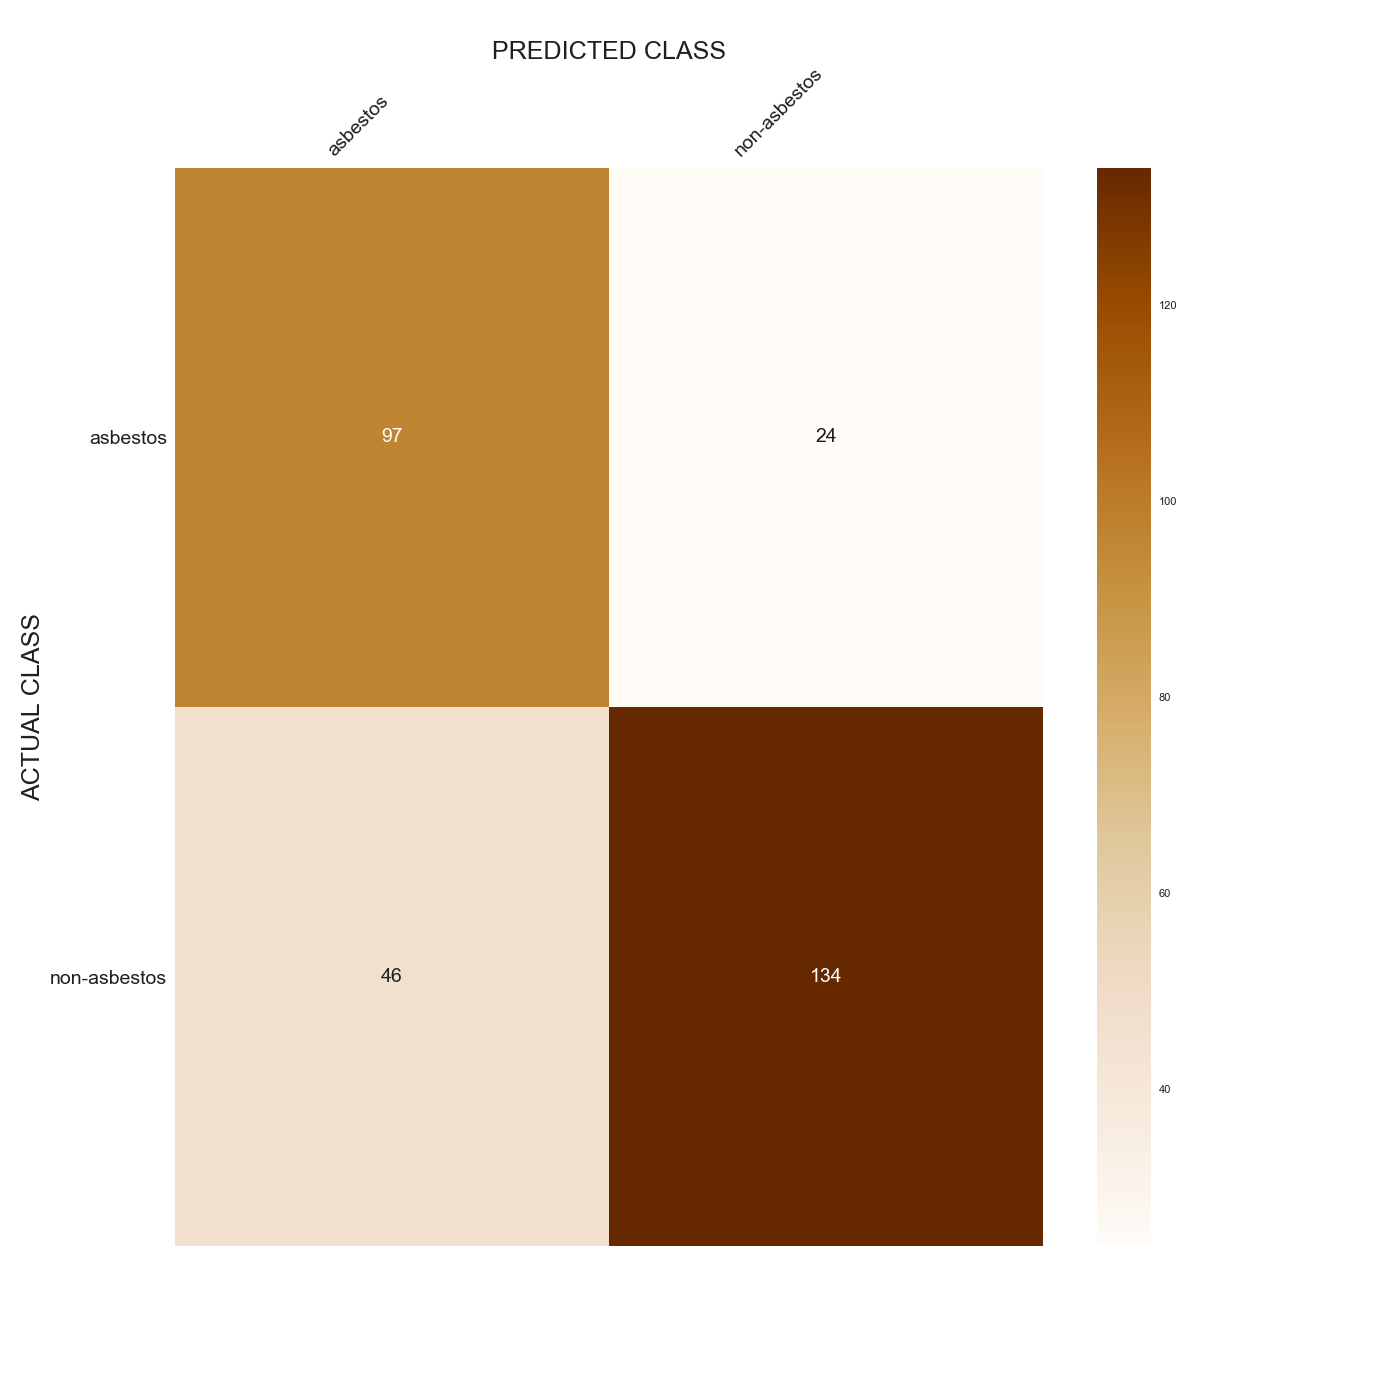
\includegraphics[width=.46\textwidth]{images/chapter5/cnn-basic-cm.png}
}
\caption{Confusion matrix of the CNN\_basic shows that the learning seems to be correct with images seperated into the two classes of asbestos and non-asbestos.}
\label{fig:cnn-basic-cm}
\end{figure}


From the confusion matrix, we can deduce type I and type II errors. Type I errors are false positives which is equivalent to a false alarm. In case of asbestos, it is better to classify wrongly some structures as asbestos than missing them which would be a type II error or a miss. Recall shows how many positive samples were actually classified as positive which in our case should be as near to 100\% as possible because it brings the type II error in relation to the overall positive samples. Recall is at 80.17\%. Precision on the other hand, how many of the predicted positive sample indeed are positive. If that number is lower, it is less severe because it simply means that more samples were classified as containing asbestos than really is the case (false alarm). Precision is at 67.83\%








%%%%%%%%%%%%%%%%%%%%%%%%%%%%%%%%%%%%%%%%%%%
%%%%%%%%%%%%%%%    ALEXNET    %%%%%%%%%%%%%%%%%%%%
%%%%%%%%%%%%%%%%%%%%%%%%%%%%%%%%%%%%%%%%%%%






\subsection{AlexNet}

AlexNet was optimized with grid search and additionally with SigOpt. With grid search the best accuracy is 81.06\% as seen in table \ref{tbl:alexnet-baseline}. It was achieved with a learning rate of 0.0001 and a learning rate decay of 20. Interestingly the SigOpt also achieved the same accuracy with a learning rate of 0.038984, a momentum of 0.073145 and a weight decay of 0.004074 as seen in table \ref{tbl:alexnet-baseline}.


\begin{table*}[h]
    \ra{1.3}
    \caption{Accuracy (\%) for several learning rates and lr-decays for AlexNet as a baseline.}
    \centering
    \begin{small}
    \textsc{
      \resizebox{0.99\textwidth}{!}{%
      \begin{tabular}{rcclcclcc}
      \toprule 
      & \multicolumn{2}{c}{Learning-Rate decay: 10} && %
        \multicolumn{2}{c}{Learning-Rate decay: 15} && %
        \multicolumn{2}{c}{Learning-Rate decay: 20} \\
      \cmidrule{2-3} \cmidrule{5-6}  \cmidrule{8-9}
      & learning rate & accuracy  && %
        learning rate & accuracy  && %
        learning rate & accuracy  \\ 
      \midrule
      AlexNet        & 0.1 & 59.80\%  &&  0.1 & 59.80\% &&  0.1 & 60.47\% \\
      AlexNet        & 0.05 & 59.80\%  &&  0.05 & 59.80\% && 0.05 & 59.80\% \\
      AlexNet        & 0.01 & 59.80\%  &&  0.01 & 59.80\% &&  0.01 & 59.80\% \\
      AlexNet        & 0.005 & 59.80\%  &&  0.005 & 59.80\% &&  0.005 & 59.80\% \\
      AlexNet        & 0.001 & 74.75\%  &&  0.001 & 77.74\% &&  0.001 & 78.74\% \\
      AlexNet        & 0.0005 & 78.74\%  &&  0.0005 & 80.40\% &&  0.0005 & 76.74\% \\
      AlexNet        & 0.0001 & 74.75\%  &&  0.0001 & 80.07\% &&  \textbf{0.0001} & \textbf{81.06\%} \\
    \bottomrule
    \end{tabular}}
    }
    \end{small}
    %\end{center}
    \vspace{-3.9mm}
    \label{tbl:alexnet-baseline}
\end{table*}

\subsection{Transfer learning on AlexNet}

When using weights from pre-training on ImageNet, the overall accuracy does get slightly better, although the increase of 0.6645\% could be due to chance. In order to show if pre-training really helps with AlexNet, each model has been run 5 times and the results are averaged as seen in Table \ref. A t-test has been run to show it's significance [NEEDS TO BE DONE]

\begin{table}[h] \centering
\ra{1.3}
\caption{Hyper parameters for Alexnet optimized with SigOpt and without pre-training}
\resizebox{0.99\textwidth}{!}{%
\begin{tabular}{@{}rrrrrrr@{}}
\toprule & learning rate & momentum & weight\_decay & lr-decay & accuracy & $\Delta$ \\
\midrule
AlexNet     from scratch    & 0.038498 & 0.073146 &  0.004074 & 20 & 81.0631\%  &         \\
AlexNet     pre-trained    & 0.034288 & 0.409378 &  0.005959 & 20 & 81.7276\%  & + 0.6645\\
\bottomrule
\end{tabular}}
\label{tbl:AlexNetBaseline}
\end{table}

\begin{table}[h] \centering
\ra{1.3}
\caption{Hyper parameters for Alexnet optimized with SigOpt and without pre-training}
\resizebox{0.99\textwidth}{!}{%
\begin{tabular}{@{}rrrrrrr@{}}
\toprule & learning rate & momentum & weight\_decay & lr-decay & accuracy & $\Delta$ \\
\midrule
AlexNet     from scratch    & 0.038498 & 0.073146 &  0.004074 & 20 & 78.61$\pm$1.16  & -     \\
AlexNet     pre-trained    & 0.034288 & 0.409378 &  0.005959 & 20 & 79.67$\pm$1.08  & - \\
AlexNet from scratch (Adam Optimizer) & 0.038498 & Adam & Adam & 20 & 59.80$\pm$0.0 & \\
\bottomrule
\end{tabular}}
\label{tbl:AlexNetMultiRun}
\end{table}

In Figure \ref{fig:alexnet-graph} we see the training and validations accuracies plotted over epochs. It can be observed that convergence is not faster with pre-training than without pre-training. Both final accuracies are almost identical. The gray vertical lines separate the graph into segments with different learning rates. So the learning rate decay happens a first time at epoch 20 and a second time at epoch 40. Convergence can be easily observed when the validation accuracy does not change anymore. Another important thing to notice is that validation and training accuracies are quite near to each other. This means that during training no severe overfitting occurred and that the validation set and train set are indeed very representative of each other. Since the final accuracy is also very near to these values it is save to say that validation and test sets are good representations of the test set and that generalizability has low variance [IF GENERALIZABILITY CAN HAVE A VARIANCE AT ALL... TODO: READ IT UP].

\begin{figure}[h]
\centering
\subfigure{
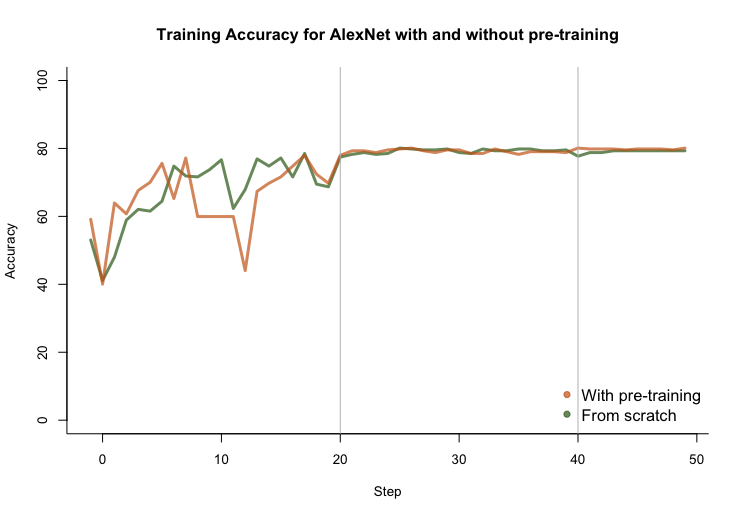
\includegraphics[width=.46\textwidth]{images/chapter5/TL/AlexNet/TA-AlexNet.png}
}
\subfigure{
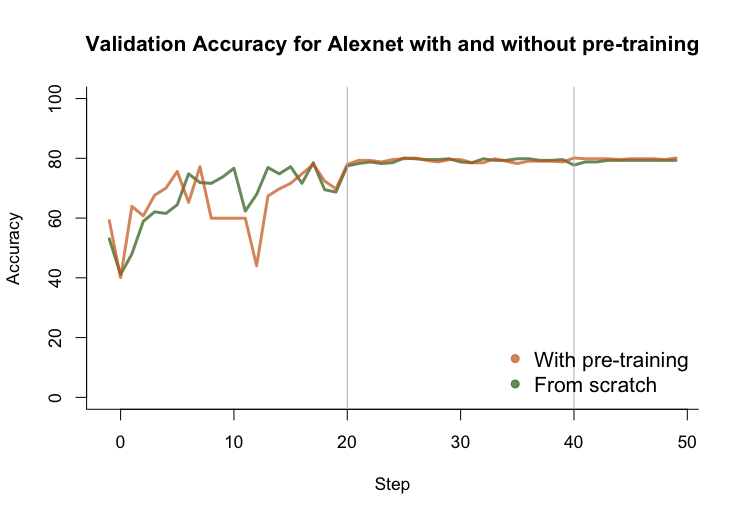
\includegraphics[width=.46\textwidth]{images/chapter5/TL/AlexNet/VA-AlexNet.png}
}
\caption{No clear difference can be observed between the pre-trained AlexNet and the not pre-trained AlexNet. Both converge roughly equally and reach almost the same final accuracy.}
\label{fig:alexnet-graph}
\end{figure}

In Figure \ref{fig:alexnet-cm} the confusion matrix of the final test set is shown for both models (pre-trainend and non pre-trained). 

\begin{figure}[h]
\centering
\subfigure{
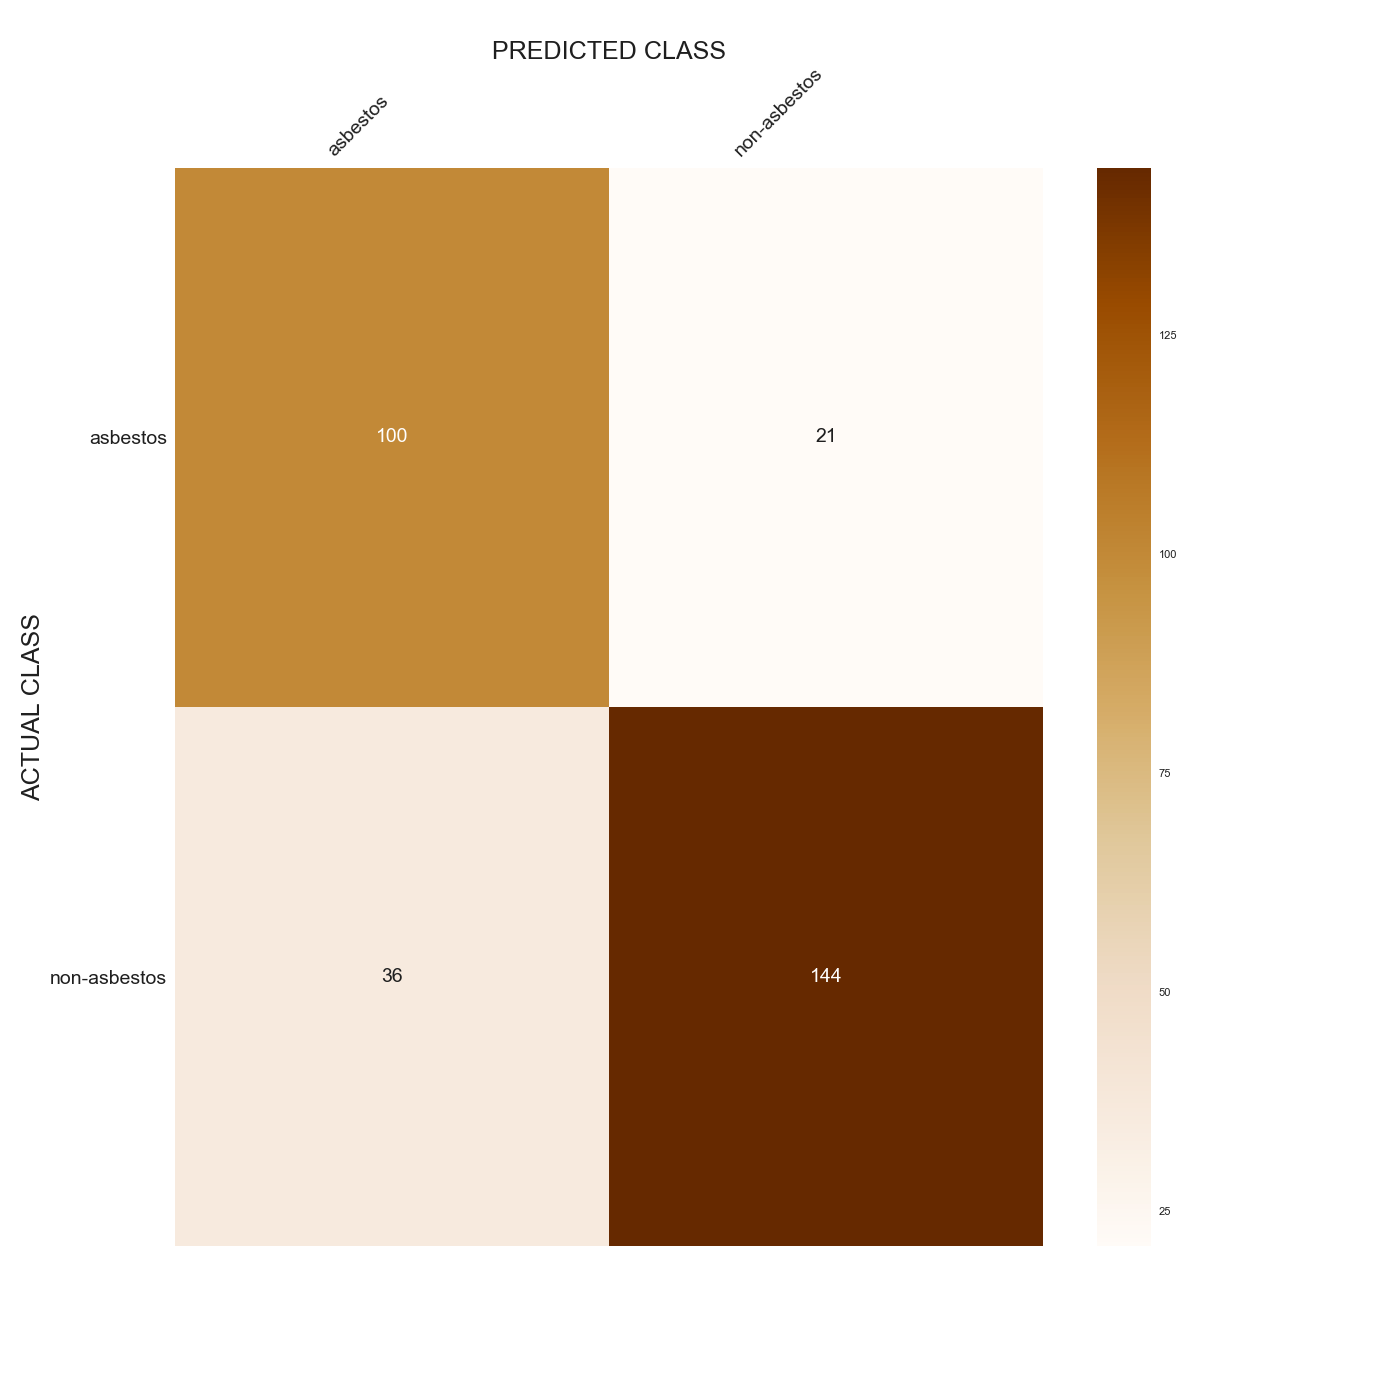
\includegraphics[width=.46\textwidth]{images/chapter5/TL/AlexNet/cm-alexnet.png}
}
\subfigure{
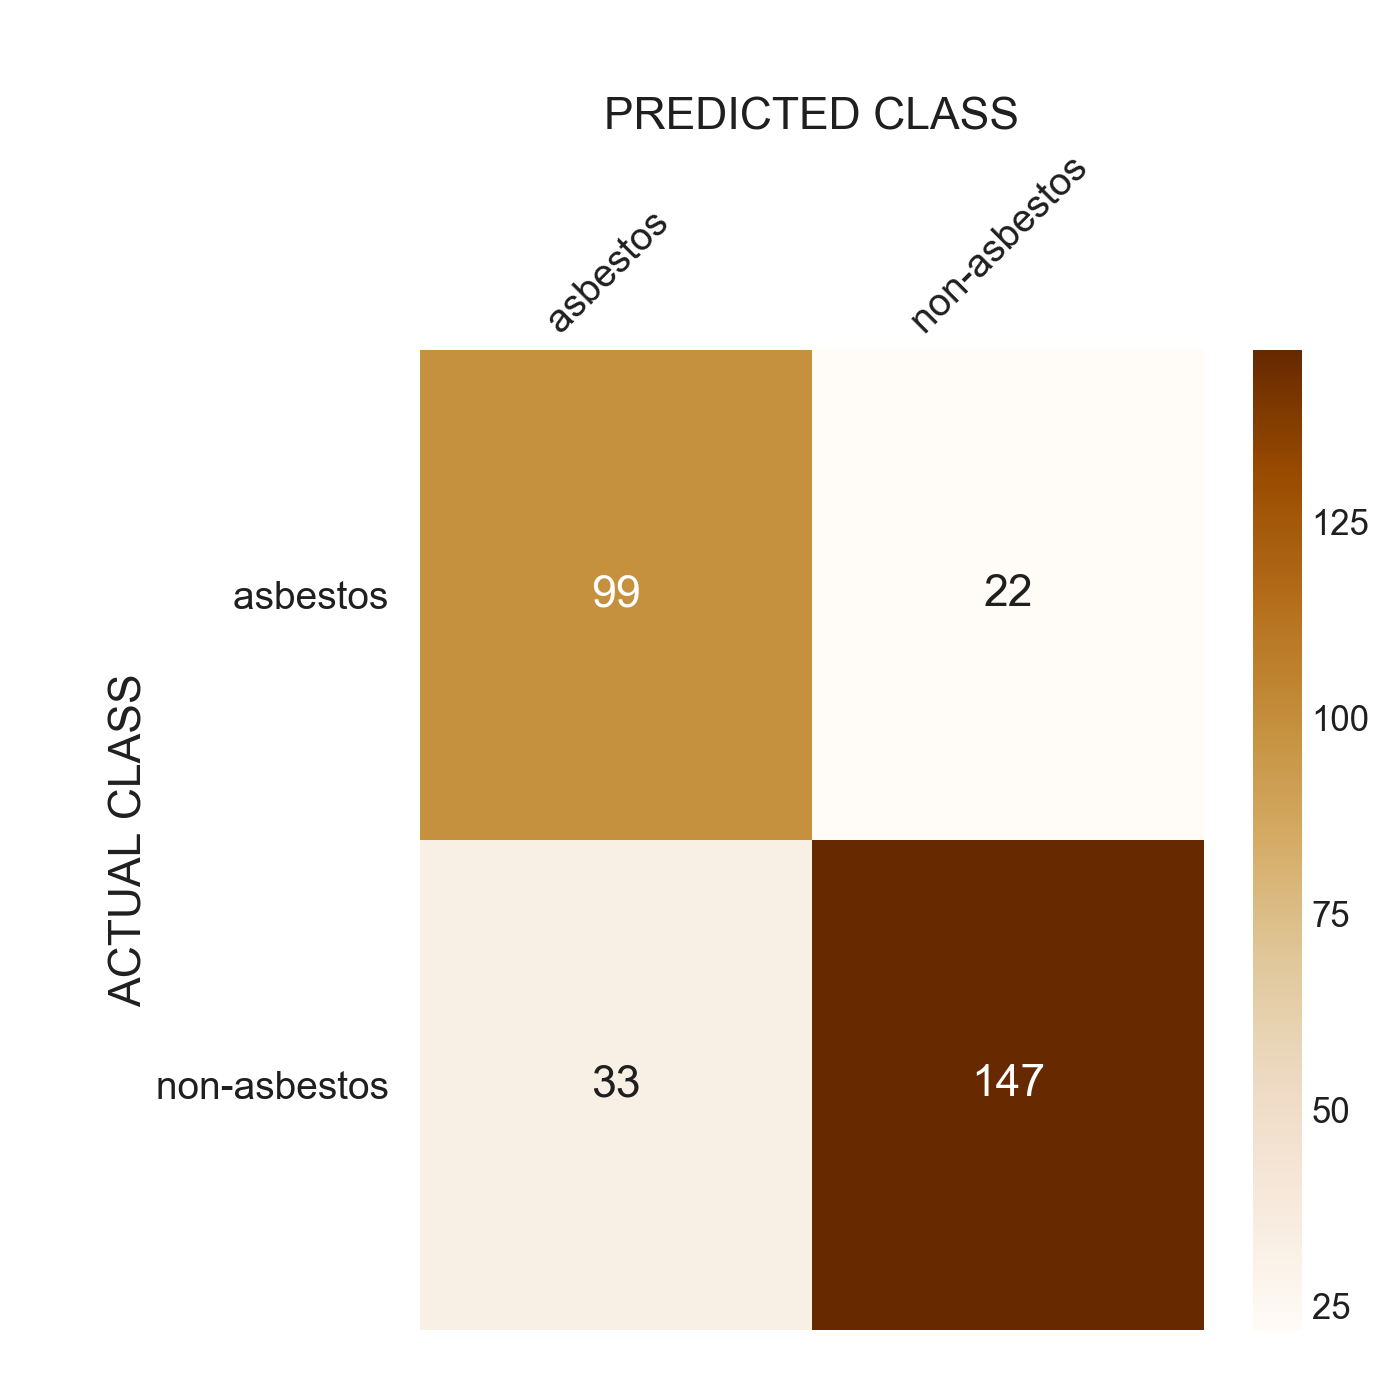
\includegraphics[width=.46\textwidth]{images/chapter5/TL/AlexNet/cm-alexnet-pre.png}
}
\caption{Confusion matrix from the model trained from scratch on the left side, and the model with pre-trained weights on the right.}
\label{fig:alexnet-cm}
\end{figure}








%%%%%%%%%%%%%%%%%%%%%%%%%%%%%%%%%%%%%%%%%%%
%%%%%%%%%%%%%%%%    VGG    %%%%%%%%%%%%%%%%%%%%%
%%%%%%%%%%%%%%%%%%%%%%%%%%%%%%%%%%%%%%%%%%%








\section{VGG}

For the following VGG architectures, the hyperparameter optimization was done with SigOpt. Every architecture was performed with and without batch normalization as well as with and without pre-training. Table \ref{tbl:VGG_overview} summarizes the results for the VGG architectures with the common depths of 11, 13 and 16. These are all the best achieved values in one run only.

\begin{table}[H] \centering
\ra{1.3}
\caption{Hyper parameters for VGG11, VGG13 and VGG16 with and without batch normalization (bn) optimized with SigOpt. First row of each grouping shows training the architecture from scratch. Second row of each grouping shows training with pre-trained weights from ImageNet}
\resizebox{0.99\textwidth}{!}{%
\begin{tabular}{@{}rrrrrrr@{}}
\toprule & learning rate & momentum & weight\_decay & lr-decay & accuracy & $\Delta$ \\
\midrule
VGG11 from scratch		& 0.026981 & 0.743190 & 0.01 & 20 & 80.7309\%  &         \\
VGG11 pre-trained		& 0.006787 & 0.696714 & 0.01 & 20 & 88.0399\%  & +7.309 \\
\midrule
VGG11\_bn  from scratch	&     0.059343 & 0.120718 &  0.009362 & 20 & 81.0631\%  &         \\
\textbf{VGG11\_bn pre-trained}	& \textbf{0.022571} & \textbf{0.383537} &  \textbf{0.001733} & \textbf{20} &  \textbf{89.7010\%} & \textbf{+8.6379} \\
\midrule
VGG13 from scratch		& 0.033844 & 0.257538 &  0.01 & 20 & 81.0631\%  &         \\
VGG13 pre-trained    	& 0.020012 & 0.193932 & 0.01 & 20 & 88.7043\%  & +7.6412 \\
\midrule
VGG13\_bn from scratch    			& 0.054173 & 0.643504 &  0.003223 & 20 & 81.7276\%  &         \\
\textbf{VGG13\_bn  pre-trained}    &  \textbf{0.093533} & \textbf{0.041074} &  \textbf{0.009734} & \textbf{20} & \textbf{90.3655\%}  & \textbf{+8.6379} \\
\midrule
VGG16 from scratch   	& 0.019590 & 0.383297 &  0.00001 & 20 & 81.7276\%  &         \\
\textbf{VGG16 pre-trained}    	& \textbf{0.009735} & \textbf{0.529937} & \textbf{0.01} & \textbf{20} & \textbf{90.6977\%}  & \textbf{+8.9701} \\
\midrule
VGG16\_bn from scratch	&     0.031702 & 0.370868 &  0.006288 & 20 & 83.0565\%  &         \\
VGG16\_bn pre-trained		&     0.083995 & 0.242109 &  0.002634 & 20 & 89.0366\%  & +5.9801 \\
\bottomrule
\end{tabular}}
\label{tbl:VGG_overview}
\end{table}

It can be seen that transfer learning helps in every single case and yields better performance by roughly additional 8\%. Also VGG performs generally better with batch normalization with one exception for VGG16 with pre-trained weights. This architecture outperformed its batch norm counterpart by 1.66\% which could be purely by chance. VGG13 with batch normalization seems to perform very well, although by a very small margin, since it is also less complex than VGG16, it will be used for further investigation. First, it is run three times with the found hyper parameters and then averaged as seen in Table \ref{tbl:VGG_averaged}. Since the values mentioned in Table \ref{tbl:VGG_overview} are the best values from 30 runs, it does not surprise that they are higher than the averaged values from Table \ref{tbl:VGG_averaged}.

\begin{table}[H] \centering
\ra{1.3}
\caption{Running the best VGG architecture three times with the found hyperparameters and averaging across the total of runs. }
\resizebox{0.99\textwidth}{!}{%
\begin{tabular}{@{}rrrrrrr@{}}
\toprule & learning rate & momentum & weight\_decay & lr-decay & accuracy & $\Delta$ \\
\midrule
VGG13\_bn from scratch	& 0.054173 	& 0.643504 	& 0.003223 	& 20 	& 81.0631\% $\pm$ 0.5425 &         \\
VGG13\_bn pre-trained		& 0.093533 	& 0.041074 	& 0.009734 	& 20 	& 88.0399\% $\pm$ 0.7176 & +6.9768\\
\bottomrule
\end{tabular}}
\label{tbl:VGG_averaged}
\end{table}

Looking at the training and validation graphs in Figure \ref{fig:vgg13-graph} a very similar behavior can be observed as in the previous graphs of the AlexNet architectures. Training accuracy is overfitting with the pre-trained model very quickly, convergence happens within the first 20 epochs, while training from scratch needs roughly 30 epochs to converge and never catches up with the pre-trained model. For the validation graph, convergence happens for both models shortly after 20 epochs and the validation accuracy is better with pre-trained weights (87.98\%) than from scratch (79.79\%). Both values are very near the actual values obtained in the test set which again confirms the hypothesis that the validation set does represent the test set very well.

\begin{figure}[H]
\centering
\caption{Training and validation graphs for VGG13 once with pre-trained weights from ImageNet (orange) and once trained from scratch (green)}
\subfigure{
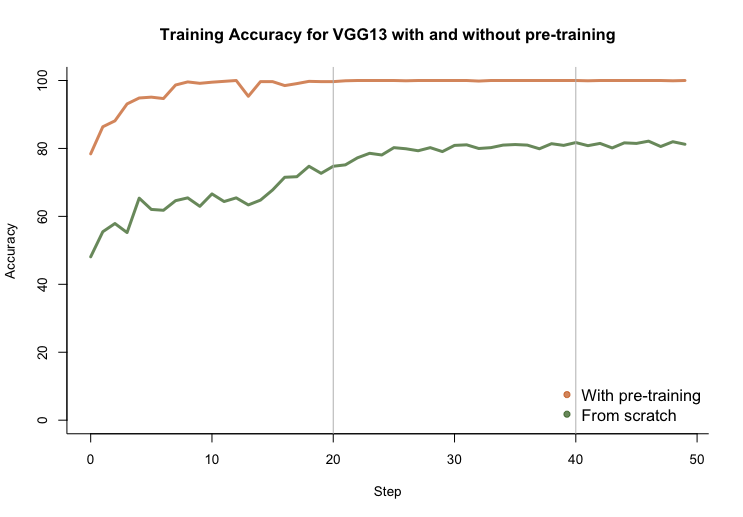
\includegraphics[width=.46\textwidth]{images/chapter5/TL/VGG13/TA-vgg13.png}
}
\subfigure{
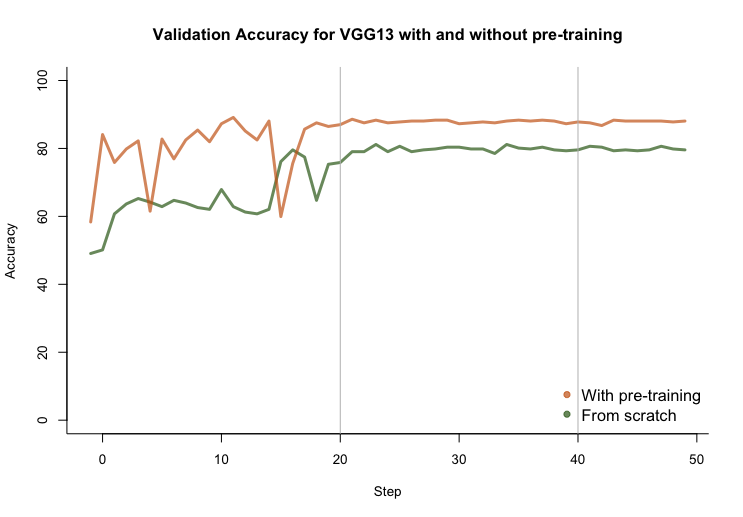
\includegraphics[width=.46\textwidth]{images/chapter5/TL/VGG13/VA-vgg13.png}
}
\label{fig:vgg13-graph}
\end{figure}

\subsection{VGG visualization}

In order to shed some light into what is going on, visualizing the CNN layers can show what kind of input images activate a specific filter and thus lead to a certain classification. Several hundred visualizations were checked at different layers for VGG13\_bn with and without transfer learning. In Figure \ref{fig:vgg13_pretrained_filters} 16 interesting layer activations from the pretrained model are shown. Filters that resembled rocks, background or fiber-like structures were selected from 4 different layers.

\begin{figure}[H]
\centering
\caption{Each line represents one convolution layer in the VGG13\_bn pre-trained architecture in ascending order. Four interesting activations are shown per layer starting at layer 2, layer 4, layer 7 and layer 9.}
\subfigure{
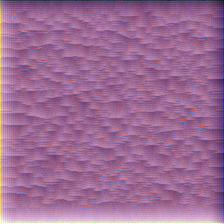
\includegraphics[width=.23\textwidth]{images/chapter5/vgg13-bn-pre/l3-f0.jpg}
}
\subfigure{
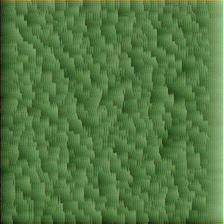
\includegraphics[width=.23\textwidth]{images/chapter5/vgg13-bn-pre/l3-f1.jpg}
}
\subfigure{
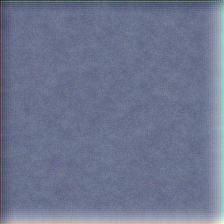
\includegraphics[width=.23\textwidth]{images/chapter5/vgg13-bn-pre/l3-f2.jpg}
}
\subfigure{
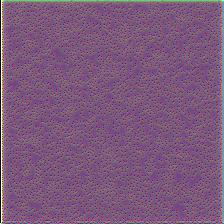
\includegraphics[width=.23\textwidth]{images/chapter5/vgg13-bn-pre/l3-f3.jpg}
}

\subfigure{

\includegraphics[width=.23\textwidth]{images/chapter5/vgg13-bn-pre/l10-f0.jpg}
}
\subfigure{
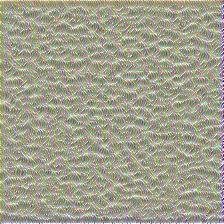
\includegraphics[width=.23\textwidth]{images/chapter5/vgg13-bn-pre/l10-f1.jpg}
}
\subfigure{
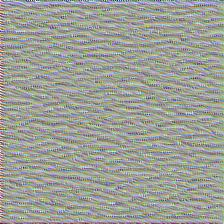
\includegraphics[width=.23\textwidth]{images/chapter5/vgg13-bn-pre/l10-f2.jpg}
}
\subfigure{
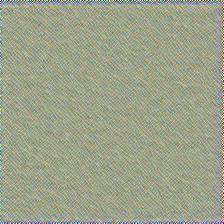
\includegraphics[width=.23\textwidth]{images/chapter5/vgg13-bn-pre/l10-f3.jpg}
}

\subfigure{

\includegraphics[width=.23\textwidth]{images/chapter5/vgg13-bn-pre/l21-f0.jpg}
}
\subfigure{
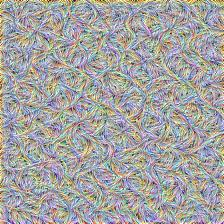
\includegraphics[width=.23\textwidth]{images/chapter5/vgg13-bn-pre/l21-f1.jpg}
}
\subfigure{

\includegraphics[width=.23\textwidth]{images/chapter5/vgg13-bn-pre/l21-f2.jpg}
}
\subfigure{

\includegraphics[width=.23\textwidth]{images/chapter5/vgg13-bn-pre/l21-f3.jpg}
}

\subfigure{

\includegraphics[width=.23\textwidth]{images/chapter5/vgg13-bn-pre/l28-f0.jpg}
}
\subfigure{
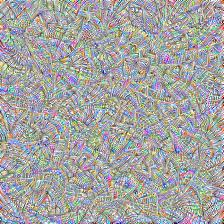
\includegraphics[width=.23\textwidth]{images/chapter5/vgg13-bn-pre/l28-f1.jpg}
}
\subfigure{

\includegraphics[width=.23\textwidth]{images/chapter5/vgg13-bn-pre/l28-f2.jpg}
}
\subfigure{

\includegraphics[width=.23\textwidth]{images/chapter5/vgg13-bn-pre/l28-f3.jpg}
}
\label{fig:vgg13_pretrained_filters}
\end{figure}

It can be very well observed that with increasing depth of the network more complex patterns are learned. In Figure \ref{fig:vgg13_app_pretrained_filters} in the Appendix, four images are shown for every layer in the architecture. The first layer learns only to spot plain colors, but already the second layer starts to look for vertical and horizontal rock-like patterns, as seen in Figure \ref{fig:vgg13_fromscratch_filters}. Some of the filters don't resemble anything from the training set but still have a high degree of pattern. These patterns were transferred over from ImageNet and adapted through 50 epochs of learning. Figure \ref{fig:vgg13_fromscratch_filters} shows four layers of the pre-trained VGG13 architectue.

\begin{figure}[H]
\centering
\caption{Each line represents one convolution layer in the VGG13\_bn architecture which was trained from scratch in ascending order. Four interesting activations are shown per layer starting at layer 2, layer 4, layer 7 and layer 9.}
\subfigure{
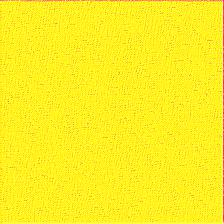
\includegraphics[width=.23\textwidth]{images/chapter5/vgg13-bn/l3-f0.jpg}
}
\subfigure{
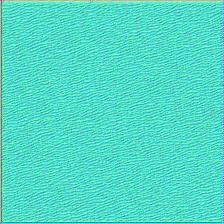
\includegraphics[width=.23\textwidth]{images/chapter5/vgg13-bn/l3-f1.jpg}
}
\subfigure{
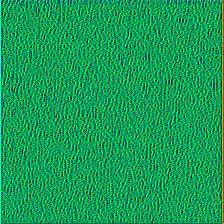
\includegraphics[width=.23\textwidth]{images/chapter5/vgg13-bn/l3-f2.jpg}
}
\subfigure{
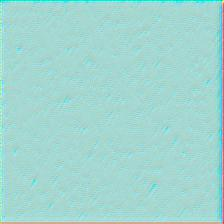
\includegraphics[width=.23\textwidth]{images/chapter5/vgg13-bn/l3-f3.jpg}
}

\subfigure{
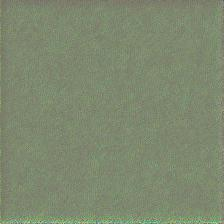
\includegraphics[width=.23\textwidth]{images/chapter5/vgg13-bn/l10-f0.jpg}
}
\subfigure{
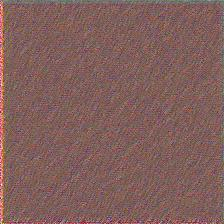
\includegraphics[width=.23\textwidth]{images/chapter5/vgg13-bn/l10-f1.jpg}
}
\subfigure{
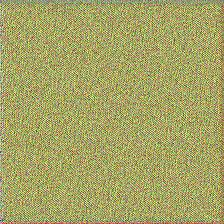
\includegraphics[width=.23\textwidth]{images/chapter5/vgg13-bn/l10-f2.jpg}
}
\subfigure{
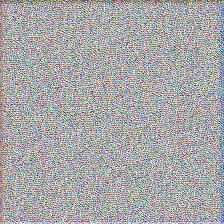
\includegraphics[width=.23\textwidth]{images/chapter5/vgg13-bn/l10-f3.jpg}
}

\subfigure{

\includegraphics[width=.23\textwidth]{images/chapter5/vgg13-bn/l21-f0.jpg}
}
\subfigure{

\includegraphics[width=.23\textwidth]{images/chapter5/vgg13-bn/l21-f1.jpg}
}
\subfigure{

\includegraphics[width=.23\textwidth]{images/chapter5/vgg13-bn/l21-f2.jpg}
}
\subfigure{

\includegraphics[width=.23\textwidth]{images/chapter5/vgg13-bn/l21-f3.jpg}
}

\subfigure{

\includegraphics[width=.23\textwidth]{images/chapter5/vgg13-bn/l28-f0.jpg}
}
\subfigure{

\includegraphics[width=.23\textwidth]{images/chapter5/vgg13-bn/l28-f1.jpg}
}
\subfigure{

\includegraphics[width=.23\textwidth]{images/chapter5/vgg13-bn/l28-f2.jpg}
}
\subfigure{

\includegraphics[width=.23\textwidth]{images/chapter5/vgg13-bn/l28-f3.jpg}
}
\label{fig:vgg13_fromscratch_filters}
\end{figure}

It is very interesting to observe that no complex patterns can be found in these layer activations instead, there is a lot of noise in the images. Although rock like structures could be interpreted into these visualizations, fiber like structures are missing completely.

Applying Grad-CAM and heatmap visualizations can show important regions of the image that correspond to a certain classification. These areas are colored in deep red to orange, whereas areas that did not contribute are colored in blue to violet. Figure \ref{fig:vgg13_pre_heatmap} shows two Gad-CAM visualizations from different layers. In the first row the second convolution layer is shown with the network recognizing rather fine-grained regions detected by the low-level feature maps. The second row shows the last convolution layer where high-level feature maps are captured.

\begin{figure}[H]
\centering
\caption{Grad-Cam and heatmap visualizations are shown for the pre-trained architectures for layers 3 and 31}
\subfigure{
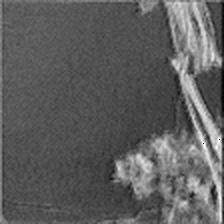
\includegraphics[width=.25\textwidth]{images/chapter5/vgg13-bn-pre/7-Cam-Grayscale.png}
}
\subfigure{
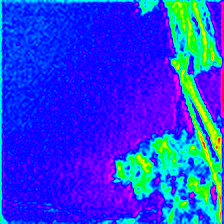
\includegraphics[width=.25\textwidth]{images/chapter5/vgg13-bn-pre/7-Cam-Heatmap.png}
}
\subfigure{
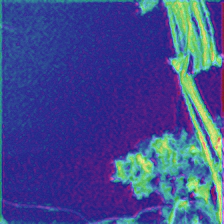
\includegraphics[width=.25\textwidth]{images/chapter5/vgg13-bn-pre/7-Cam-Image.png}
}

\subfigure{
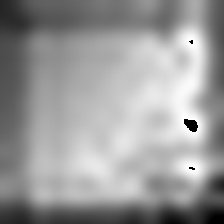
\includegraphics[width=.25\textwidth]{images/chapter5/vgg13-bn-pre/31-Cam-Grayscale.png}
}
\subfigure{
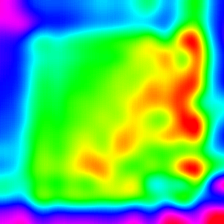
\includegraphics[width=.25\textwidth]{images/chapter5/vgg13-bn-pre/31-Cam-Heatmap.png}
}
\subfigure{
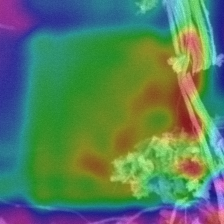
\includegraphics[width=.25\textwidth]{images/chapter5/vgg13-bn-pre/31-Cam-Image.png}
}
\label{fig:vgg13_pre_heatmap}
\end{figure}

In Figure \ref{fig:vgg13_heatmap} the same Grad-CAM visualizations are shown at the same layers for the model trained from scratch. It can be easily seen that although the low-level features are still similar the last convolution layer yields completely different results.

\begin{figure}[H]
\centering
\caption{Grad-Cam and heatmap visualizations are shown for the pre-trained architectures for layers 3 and 31}
\subfigure{
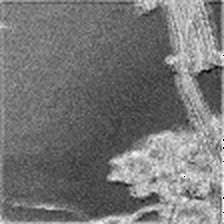
\includegraphics[width=.25\textwidth]{images/chapter5/vgg13-bn/7-Cam-Grayscale.png}
}
\subfigure{
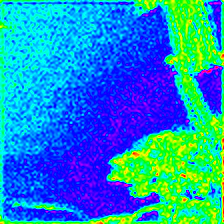
\includegraphics[width=.25\textwidth]{images/chapter5/vgg13-bn/7-Cam-Heatmap.png}
}
\subfigure{
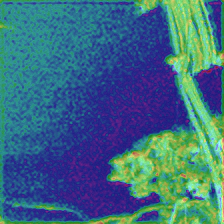
\includegraphics[width=.25\textwidth]{images/chapter5/vgg13-bn/7-Cam-Image.png}
}


\subfigure{
\includegraphics[width=.25\textwidth]{images/chapter5/vgg13-bn/31-Cam-Grayscale.png}
}
\subfigure{
\includegraphics[width=.25\textwidth]{images/chapter5/vgg13-bn/31-Cam-Heatmap.png}
}
\subfigure{
\includegraphics[width=.25\textwidth]{images/chapter5/vgg13-bn/31-Cam-Image.png}
}
\label{fig:vgg13_heatmap}
\end{figure}











%%%%%%%%%%%%%%%%%%%%%%%%%%%%%%%%%%%%%%%%%%%
%%%%%%%%%%%%%%%%%    RESNET    %%%%%%%%%%%%%%%%%%%
%%%%%%%%%%%%%%%%%%%%%%%%%%%%%%%%%%%%%%%%%%%




\section{ResNet}

ResNet18 and ResNet34 were both optimized with SigOpt only. For each hyper parameter 10 runs were conducted summing up to 30 runs. It was used for training the architecture from scratch and with pre-trained weights. Table \ref{tbl:ResNet_overview} shows a summary of the optimization process with the best accuracies and the delta between the pre-trained model and the model trained from scratch.

\begin{table}[h] \centering
\ra{1.3}
\caption{Hyper parameters for ResNet18 and ResNet34 optimized with SigOpt. First row shows hyperparameters training the architecture from scratch. Second row used pre-trained weights from ImageNet}
\resizebox{0.99\textwidth}{!}{%
\begin{tabular}{@{}rrrrrrr@{}}
\toprule & learning rate & momentum & weight\_decay & lr-decay & accuracy & $\Delta$ \\
\midrule
ResNet18     from scratch    & 0.033678 & 0.952630 &  0.007518 & 20 & 83.0565\%  &         \\
ResNet18     pre-trained    &     0.039918 & 0.170826 &  0.001980 & 20 & 88.0399\%  & + 4.9834\\
\midrule
ResNet34     from scratch    & 0.040323 & 0.141704 &  0.004044 & 20 & 83.0565\%  &         \\
ResNet34     pre-trained    &     0.060848 & 0.460187 &  0.000537 & 20 & 87.0431\%  & +3.9866\\
\bottomrule
\end{tabular}}
\label{tbl:ResNet18}
\end{table}

ResNet18 and ResNet34 perform equally well when trained form scratch but differ slightly when pre-trained weights from ImageNet are used. The increased gain from transfer learning for ResNet18 is thus higher and since it has less parameters, it is the preferred architecture to be further evaluated.\\

The graphs in Figure \ref{fig:resnet18-graph} show clearly that training converged much faster for the model with pre-trained weights. After only a few epochs it reached convergence while the model without pre-trained weights had to catch up over many epochs. Both models overfit strongly to the training data and yield lower results in the validation and test sets. Interestingly the validation accuracy of the model trained from scratch starts to decrease around epoch 30 although training accuracy still rises. This is considered bad and is also reflected in the final accuracies where the model without transfer learning scores around 5\% lower.

\begin{figure}[h]
\centering
\caption{Training and validation graphs for ResNet18 once with pre-trained weights from ImageNet and once trained from scratch.}
\subfigure{
\includegraphics[width=.46\textwidth]{images/chapter5/TL/ResNet18/TA-ResNet18.png}
}
\subfigure{
\includegraphics[width=.46\textwidth]{images/chapter5/TL/ResNet18/VA-ResNet18.png}
}
\label{fig:resnet18-graph}
\end{figure}

With the confusion matrix in Figure \ref{fig:resnet18-cm} we can see that the learning did not take any shortcuts and that the distinction between images with asbestos fibers and images without were clearly separated to some extent that is reflected in the overall accuracy reached. The Precision and Recall for the model trained from scratch are 77.78\% and 80.99\%, respectively. For the model with pre-trained weight, Precision and Recall are much better with 83.47\% and 87.60\%, respectively.

\begin{figure}[h]
\centering
\caption{On the left: confusion matrix from model trained from scratch. On the right trained with transfer learning applied.}
\subfigure{
\includegraphics[width=.46\textwidth]{images/chapter5/TL/ResNet18/cm-resnet18.png}
}
\subfigure{
\includegraphics[width=.46\textwidth]{images/chapter5/TL/ResNet18/cm-resnet18-pre.png}
}
\label{fig:resnet18-cm}
\end{figure}











%%%%%%%%%%%%%%%%%%%%%%%%%%%%%%%%%%%%%%%%%%%
%%%%%%%%%%%%%%%    DENSENET121    %%%%%%%%%%%%%%%%%
%%%%%%%%%%%%%%%%%%%%%%%%%%%%%%%%%%%%%%%%%%%



\section{Densenet121}

Densenet121 and densenet169 were both optimized with SigOpt only. For each hyper parameter 10 runs were conducted summing up to 30 runs. It was used for training the architecture from scratch and with pre-trained weights. Table \ref{tbl:Densenet121_overview} shows a summary of the optimization process with the best accuracies and the delta between the pre-trained model and the model trained from scratch.

\begin{table}[h] \centering
\ra{1.3}
\caption{Hyper parameters for densenet121 optimized with SigOpt. First row shows hyperparameters training the architecture from scratch. Second row used pre-trained weights from ImageNet}
\resizebox{0.99\textwidth}{!}{%
\begin{tabular}{@{}rrrrrrr@{}}
\toprule & learning rate & momentum & weight\_decay & lr-decay & accuracy & $\Delta$ \\
\midrule
Densenet121     from scratch    & 0.035925 & 0.057618 &  0.009241 & 20 & 86.0465\%  &         \\
Densenet121     pre-trained    &     0.018489     & 0.369998 &  0.004963 & 20 & 88.3721\%  & +2.3256\\
\midrule
Densenet169 from scratch    & 0.005812 & 0.777249 & 0.006999  & 20 & 85.3821\%  &         \\
Densenet169 pre-trained    & 0.006347 & 0.447591 & 0.005180 & 20 & 89.3688\%  & +3.9867\\
\bottomrule
\end{tabular}}
\label{tbl:Densenet121_overview}
\end{table}

As already seen in the previous comparisons of VGG and ResNet architectues, the parameter size does not seem to play a role in this specific task. If the model is trained from scratch, densenet121 achieves slightly higher accuracies than densenet161. The opposite is true for the model trained with transfer learning where densenet169 performs slightly better. Since the difference is very small densenet121 is preferred for further investigation over the deeper densenet169 architecture.

The graphs in Figure \ref{fig:densenet121-graph} show again a very similar and alread known behavior. Convergence happens much faster with the pre-trained model.

\begin{figure}[h]
\centering
\caption{Training and validation graphs for densenet121 once with pre-trained weights from ImageNet and once trained from scratch.}
\subfigure{
\includegraphics[width=.46\textwidth]{images/chapter5/TL/Densenet121/TA-densenet121.png}
}
\subfigure{
\includegraphics[width=.46\textwidth]{images/chapter5/TL/Densenet121/VA-densenet121.png}
}
\label{fig:densenet121-graph}
\end{figure}





%%%%%%%%%%%%%%%%%%%%%%%%%%%%%%%%%%%%%%%%%%%
%%%%%%%%%%%%%%%    INCEPTIONv3   %%%%%%%%%%%%%%%%%%
%%%%%%%%%%%%%%%%%%%%%%%%%%%%%%%%%%%%%%%%%%%









\section{Inception}


Hyperparameter optimization for inception v3 was done with SigOpt and for both variants, training from scratch and training with pre-trained weights from ImageNet.

\begin{table}[h] \centering
\ra{1.3}
\caption{Hyper parameters for inception v3 optimized with SigOpt. First row shows hyperparameters training the architecture from scratch. Second row used pre-trained weights from ImageNet}
\resizebox{0.99\textwidth}{!}{%
\begin{tabular}{@{}rrrrrrr@{}}
\toprule & learning rate & momentum & weight\_decay & lr-decay & accuracy & $\Delta$ \\
\midrule
Inception v3 from scratch    & 0.070046 & 0.910505 & 0.006943 & 20 & 83.3887\%  &         \\
Inception v3 pre-trained    & 0.029269 & 0.0 & 0.006320 & 20 & 88.7043\%  & +5.3156\\
\bottomrule
\end{tabular}}
\label{tbl:Inceptionv3}
\end{table}

\section{Conclusion on Transfer Learning}

Using pre-trained weights from ImagNet increased accuracy of every single run performed on the above mentioned architectures. Apparently the learned feature representations are general enough to be of high  value regardles of the target domain. These findings align perfectly well with other research done on cross-domain transfer learning. By average ALKJJDLFKJDFLKJLKDFJ

Overfitting was often a problem and this should be addressed through cropping and randomization

At first it was very surprising that learning from scratch never caught up with the models using transfer learning from ImageNet. I was certain that given enough epochs and different runs the models from scratch should find at least equally suited feature mappings with random initialization of weights. But visualizing  some of the filters quickly made it clear that learning from scratch  with the provided dataset doesn't create elaborate feature mappings as seen from ImageNet. I argue that although the vast majority of feature mappings are absolutely useless for the asbestos classification, some feature mappings of e.g. grass or hair might be similar enough for the filter to activate maximally. Since the asbestos task is only a binary classification few of these filters are enogh to predict asbestos with a high accuracy. These elaborate feature mappings are not able to be created from scratch with a dataset of only a few hundred, partially wrongly labeled images, thus the model trained from scratch never reaches the accuracy of the pre-trained model.

